\section{ЗАДАЧІ МАРКЕТИНГОВОЇ РОЗВІДКИ ТА МОДЕЛЮВАННЯ МАРКЕТИНГОВИХ КАНАЛІВ}
% Ми не створюємо канал як такий. Метою роботи є маркетингове прогнозування 
% шляхом моделювання маркетингового каналу.
%
% TODO: можливо, заголовок треба буде змінити
% TODO: додати новий сорець
\subsection{Основні проблемі розробки програмних систем}
\subsubsection{Основні поняття}
Lorem Ipsum is simply dummy text of the printing and typesetting industry. Lorem Ipsum has been the industry's standard dummy text ever since the 1500s, when an unknown printer took a galley of type and scrambled it to make a type specimen book. It has survived not only five centuries, but also the leap into electronic typesetting, remaining essentially unchanged. It was popularised in the 1960s with the release of Letraset sheets containing Lorem Ipsum passages, and more recently with desktop publishing software like Aldus PageMaker including versions of Lorem Ipsum.
% TODO: програмна інженерія
% TODO: програмне забезпечення
% TODO: системна вимога
% TODO: програмний засіб
% TODO: системні вимоги
% TODO: проблемна область  
\subsubsection{Необхідність створення ПС}
Lorem Ipsum is simply dummy text of the printing and typesetting industry. Lorem Ipsum has been the industry's standard dummy text ever since the 1500s, when an unknown printer took a galley of type and scrambled it to make a type specimen book. It has survived not only five centuries, but also the leap into electronic typesetting, remaining essentially unchanged. It was popularised in the 1960s with the release of Letraset sheets containing Lorem Ipsum passages, and more recently with desktop publishing software like Aldus PageMaker including versions of Lorem Ipsum.
% TODO: системні вимоги
\subsubsection{Процес розробки ПЗ}
Lorem Ipsum is simply dummy text of the printing and typesetting industry. Lorem Ipsum has been the industry's standard dummy text ever since the 1500s, when an unknown printer took a galley of type and scrambled it to make a type specimen book. It has survived not only five centuries, but also the leap into electronic typesetting, remaining essentially unchanged. It was popularised in the 1960s with the release of Letraset sheets containing Lorem Ipsum passages, and more recently with desktop publishing software like Aldus PageMaker including versions of Lorem Ipsum.
% TODO: МЖЦ, методології
\subsubsection{Нотація, що використовується}
Lorem Ipsum is simply dummy text of the printing and typesetting industry. Lorem Ipsum has been the industry's standard dummy text ever since the 1500s, when an unknown printer took a galley of type and scrambled it to make a type specimen book. It has survived not only five centuries, but also the leap into electronic typesetting, remaining essentially unchanged. It was popularised in the 1960s with the release of Letraset sheets containing Lorem Ipsum passages, and more recently with desktop publishing software like Aldus PageMaker including versions of Lorem Ipsum.
% TODO: UML, IDEF*

\subsection{Маркетингові інформаційні системи}

\subsubsection{Огляд МІС} % TODO: додати цю абревіацію до відповідного розділу
% TODO: що це таке, навіщо воно потрібно, складові частини та їх призначення, 4Р
За визначенням Американської асоціації маркетингу, {\it маркетинг} --- це діяльність, сукупність інститутів і процесів, що забезпечують створення, інформування, доставку та обмін пропозицій, що мають цінність для споживачів, клієнтів, партнерів і суспільства в цілому \cite{kotler14}. Оскільки продажі є головним джерелом прибутку, компанії будують свою структуру та процеси з оглядом на потреби маркетингу, потреби ринку. Для прийняття ефективних маркетингових рішень, компанії організовують постійний збір та аналіз інформації про споживачів, партнерів та ринок в цілому. Для автоматизації процесу збору та аналізу, використовують системи підтримки маркетингових рішень або маркетингові інформаційні системи (МІС). Маркетингові інформаційні системи (англ. {\it marketing information systems, MkIS}) --- це сукупність людей та систем, що виконують процедури по збору, сортування, аналізу та оцінки інформації для підтримки прийняття рішень.

\begin{stdfigure}
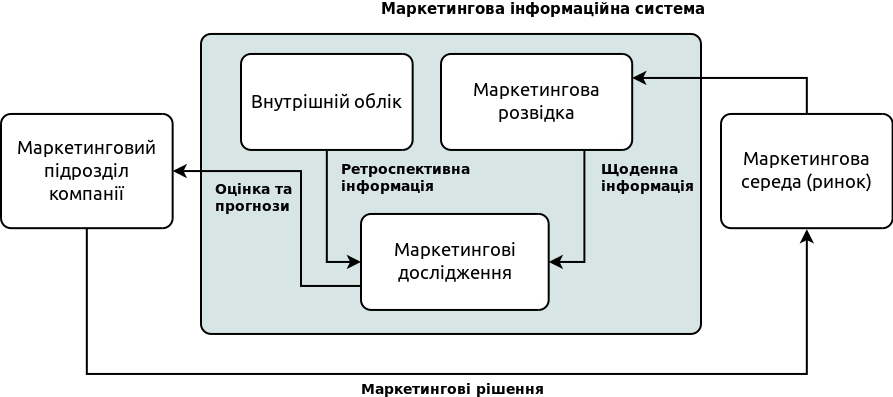
\includegraphics[width=6in]{images/mis_structure.png}
\caption{Структура МІС}
\label{fig:mis_structure}
\end{stdfigure}
 
Маркетингова інформаційна система складається з трьох частин (див рис. \ref{fig:mis_structure}): 
\begin{itemize}
\item Внутрішнього обліку.
\item Маркетингові дослідження
\item Маркетингова розвідка
\end{itemize}
% Дати визначення (із посиланням на 14-те видання)
% Вставити зображення зі схемою.
% Надати опис усім трьом частинам, остання та найдетальніша: розвідка.
% TODO: що це таке, навіщо воно потрібно, складові частини та їх призначення, 4Р

Lorem Ipsum is simply dummy text of the printing and typesetting industry. Lorem Ipsum has been the industry's standard dummy text ever since the 1500s, when an unknown printer took a galley of type and scrambled it to make a type specimen book. It has survived not only five centuries, but also the leap into electronic typesetting, remaining essentially unchanged. It was popularised in the 1960s with the release of Letraset sheets containing Lorem Ipsum passages, and more recently with desktop publishing software like Aldus PageMaker including versions of Lorem Ipsum.

\subsubsection{Маркетингова розвідка}
% TODO: Що то, нащо треба, як це робиться (моделювання, дослідження, etc), огляд наявних систем
Lorem Ipsum is simply dummy text of the printing and typesetting industry. Lorem Ipsum has been the industry's standard dummy text ever since the 1500s, when an unknown printer took a galley of type and scrambled it to make a type specimen book. It has survived not only five centuries, but also the leap into electronic typesetting, remaining essentially unchanged. It was popularised in the 1960s with the release of Letraset sheets containing Lorem Ipsum passages, and more recently with desktop publishing software like Aldus PageMaker including versions of Lorem Ipsum.

\subsubsection{Бізнес-ігри}
% TODO: що таке бізнес-ігри, навіщо вони потрібні і як реалізються
Lorem Ipsum is simply dummy text of the printing and typesetting industry. Lorem Ipsum has been the industry's standard dummy text ever since the 1500s, when an unknown printer took a galley of type and scrambled it to make a type specimen book. It has survived not only five centuries, but also the leap into electronic typesetting, remaining essentially unchanged. It was popularised in the 1960s with the release of Letraset sheets containing Lorem Ipsum passages, and more recently with desktop publishing software like Aldus PageMaker including versions of Lorem Ipsum.

\subsection{Постановка задачі}
\subsubsection{Моделювання маркетингового каналу}
%TODO: що таке концепція маркетингового каналу, основні момент структури та керування каналом.
% TODO: постановка задачі моделювання ()
Lorem Ipsum is simply dummy text of the printing and typesetting industry. Lorem Ipsum has been the industry's standard dummy text ever since the 1500s, when an unknown printer took a galley of type and scrambled it to make a type specimen book. It has survived not only five centuries, but also the leap into electronic typesetting, remaining essentially unchanged. It was popularised in the 1960s with the release of Letraset sheets containing Lorem Ipsum passages, and more recently with desktop publishing software like Aldus PageMaker including versions of Lorem Ipsum.

\subsubsection{Вимоги до програмного забезпечення}
Lorem Ipsum is simply dummy text of the printing and typesetting industry. Lorem Ipsum has been the industry's standard dummy text ever since the 1500s, when an unknown printer took a galley of type and scrambled it to make a type specimen book. It has survived not only five centuries, but also the leap into electronic typesetting, remaining essentially unchanged. It was popularised in the 1960s with the release of Letraset sheets containing Lorem Ipsum passages, and more recently with desktop publishing software like Aldus PageMaker including versions of Lorem Ipsum.
              
\subsection{Опис проблемної області}
\subsubsection{Глосарій}
В результаті аналізу проблемної області були визначені найважливіші поняття та складений глосарій:
            
\begin{enumerate}
% Написати визначення гри чи не треба?
\item {\it Бізнес-гра} --- це система моделювання, що відображає діяльність конкуруючих бізнес-організацій за допомогою теорії ігор;
\item {\it Маркетинговий канал} --- об’єкт моделювання, множина взаємопов’язаних бізнес-організацій, що утворюють ланцюг між виробником та кінцевим споживачем та надають можливість використання або споживання різних товарів чи послуг \cite{stern};
\item {\it Структура каналу} --- це сукупність бізнес-організацій, що працюють в каналі, та зв’язків між ними;
\item {\it Учасники каналу} --- це бізнес-органцізації, що входять до структури каналу і мають різні цілі;
\item {\it Керування каналом} --- це постійний процес планування та формування оптимальної структури каналу, пошуку конфліктів, що зменшують ефективність каналу та розробка методів вирішення цих конфліктів \cite{stern};
\item {\it Потік} --- це сукупність функцій, які послідовно виконуються учасниками каналу \cite{stern};
\item {\it Модератор каналу} --- це людина, або автоматизована система, що може змінювати структуру каналу;
\item {\it Адміністратор каналу} --- це людина, або автоматизована система, що керує маркетинговими каналами в бізнес-грі та може змінювати структуру каналів;
\end{enumerate}

\subsubsection{Принципи функціонування маркетингового каналу}
Маркетинговий канал --- це складний ланцюг з підприємств, які в процесі переміщення товару від виробника до кінцевого клієента, передають одне одному товар, гроші або інші ресурси. Рух ресурсів та активностей всередині каналу описується потоками, що є послідовністю виконання своїх функцій учасниками \cite{stern}. Наприклад, рух товарів (тобто потік фізичного володіння товаром) чи рух права власності на товар є потоками. В межах цих та інших потоків (всі потоки зображені на рис. \ref{fig:streams}) відбуваються всі активності в каналі. Потоки поділяються на прямі, зворотні та двосторонні. Прямі потоки йдуть від виробника до кінцевого споживача, зворотні, навпаки, від споживача до виробника, а двосторонні --- в обох напрямках. До прямих відносять: фізичне володіння, право власності, реклама. До двосторонніх: переговори, фінансування, управлення ризиками. До зворотніх потоки: замовлення, оплата. В цій роботі розглядаються потоки права власності, замовлень та оплати.
\begin{stdfigure}
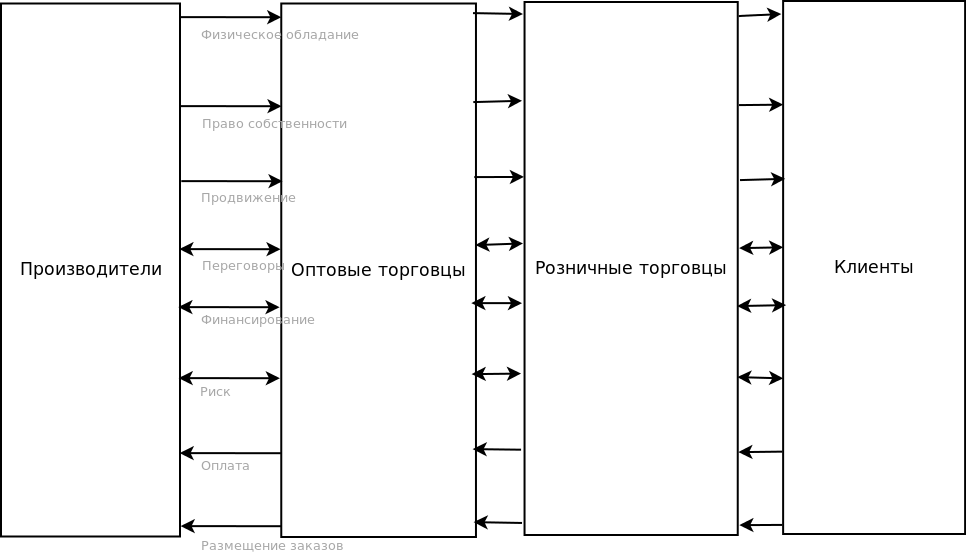
\includegraphics[width=6in]{images/streams.png}
\caption{Потоки в маркетингових каналах}
\label{fig:streams}
\end{stdfigure}

\subsubsection{Структура маркетингового каналу}

До структури маркетингового каналу входять підприємства, що поділені на чотири групи: виробники, дистриб’ютори, рітейлери та клієнти. Представники різних груп виконують різні ролі та оперують різною кількістю товару. 

Учасники каналу можуть безпосередньо співпрацювати між собою, лише якщо між ними встановлені зв’язки, що відображають потоки права власності на товар, замовлень та оплати. Зв’язки встановлюються модератором чи адміністратором каналу за наступними правилами:
\begin{itemize}
\item виробник може передавати право власності на товар тільки дистриб’юторам, а також завершує всі зворотні потоки;
\item дистриб’ютор може відправляти платежі та робити замовлення тільки виробникам, а передавати право власності на товар тільки рітейлерам;
\item рітейлер замовляє та платить тільки дистриб’юторам, а право власності на товар може передавати тільки клієнтам;
\item клієнт замовляє товар та сплачує за нього безпосередньо рітейлерам і завершує всі прямі потоки в каналі.
\end{itemize}

\subsubsection{Задачі керування маркетинговим каналом}

В процесі досягнення загальних цілей маркетингового каналу, кожне підприємство намагається досягнути власних бізнес-цілей і можуть виникнути ситуації, коли між учасниками каналу з’являються конфлікти бізнес-інтересів. Такі конфлікти приводять до некоординованої роботи учасників, а це приводить до невиконання загальної бізнес-цілі всього каналу. Щоб не допустити цього, адміністратор каналу може вводити обмеження на діяльність учасників, тим самим контролюючи їх дії. Визначимо першою задачею керування каналом знаходження рівноваги, за якої виконується загальна ціль всього каналу та кожного учасника окремо. 

Для того, щоб задовольнити вимоги споживачів, учасники каналу використовують дорогі ресурси (що можуть буди загальними): складські приміщення, транспорт, люди тощо. Важливо недопустити наявність в структурі каналу компаній, що неефективно використовують наявні потужності, наприклад: через недоліки технологічних процесів простоює дороге обладнання або учасники дублюють функції один одного. Так, сформулюємо другу задачу керування каналом: оптимізація структури каналу для більш ефективного використання ресурсів.
